\section{Discussion} 
\subsection{RQ 1: How can textual sentiment prediction be optimised?}

Two main methods of predicting the sentiment of input text have been analysed, using a bag-of-words method, and using machine learning approaches.

The lexicon based bag-of-words is based entirely on having an appropriate dataset to rank the words, since as Table \ref{lexicon:f1} shows, having rated VAD scores which follow a certain structure is key to obtaining good results. Dimensions like the Dominance and Arousal of a piece of text can be very subjective, and vary depending on what basis the dataset is judging the scores on.

The decision to use the machine learning based model for the implementation is due to having overall more stable F1 scores for each dimension, but this is only due the model having trained and tested over similar data, from the same dataset.

The use of pre-processing the data, choosing an the best classification model, and selecting appropriate sampling methods lead to the final model established in Section \ref{finalModelSection},  resulting in the highest F1 score we can obtain by trialling these methods. To answer RQ \ref{RQ1}, we can argue that out of the investigations that have been addressed, our conclusions for each of these findings can be decided as optimal, however more work can be done to explore whether the F1 score, and with it the optimality of the prediction model can be increased further.

One point which has not been addressed by this investigation is that the VAD values for each sentence are related to one another. This can be shown by the mosaic plot of the data in Figure \ref{mosaic:emo}, where we can see that the majority of the data is taken up by samples which are neutral in all three dimensions, that is, if the prediction over a sentence returns that it has neutral Valence and Arousal, then it is much more likely to have a neutral Dominance. Figure \ref{mosaic:emo} also displays the Pearson residuals for the data, which shows that for many of the classes that contain Neutral values, particularly neutral Arousal there are a lot less samples than expected when a Pearson $\chi^2$ test is performed \cite{zeileis2007residual}. This test is performed against a null hypothesis that the distribution of values are independent, and in this case it rejects this null hypothesis with a p-value of 2.22E-16.
\begin{figure}[ht]
\centering
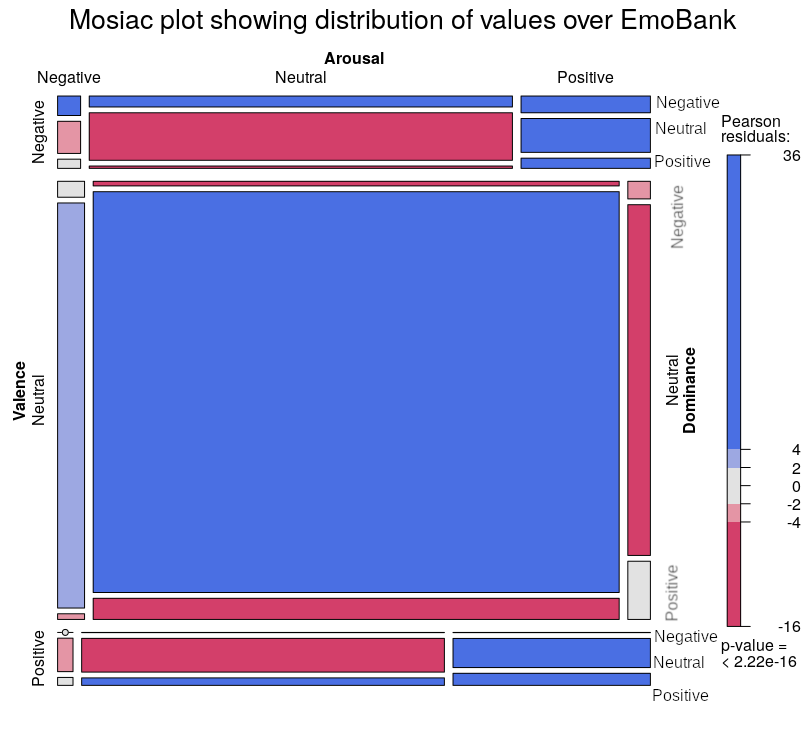
\includegraphics[scale=0.7]{graphs/mosaic_new.png}
\caption{Emobank data distribution with relationships. The Pearson residuals are the deviation from the expected frequency by a Pearson $\chi^2$ Test \cite{pearson1900x}}
\label{mosaic:emo}
\end{figure}

Because of this, a small extension investigation was done using the existing model setup as given in Section \ref{finalModelSection} to train a model to each predict a V, A, D value, given the other two as inputs, as shown in Figure \ref{model:adjust}. Since these adjustment models do not take in the input sentence, the number of feature selection and N-gram values were not needed.

\begin{figure}[ht]
\centering

\includegraphics[scale=0.6]{implementation/adjustModel.png}
\caption{Diagram showing inputs and outputs for the valence prediction model}
\label{model:adjust}
\end{figure}

These models have good F1 scores compared to the model with the sentence data, and more investigation needs to be done on how to incorporate these adjustment models into the final result. 

\begin{table}[h]
\centering
\caption{F1 scores for adjustment models}
\begin{tabular}{|l|l|}
\hline
Model & F1 Score \\ \hline
 Valence Prediction &  0.778\\
 Arousal Prediction &  0.864\\
 Dominance Prediction &  0.893\\
 \hline
\end{tabular}
\label{f1:adj}
\end{table}

\subsection{RQ 2: Is using more than 1 dimension to classify emotions useful?}

Analysing something like insight into an emotion is very subjective, and finding a good way to evaluate this has been difficult. With 60\% of the five test users agreeing with the sentiment behind the output song, it could be said that there is reason to believe that the model produces accurate results. 

Something that has an effect on the calculated song is that it is chosen from the users recent frequent listening history.
What can be done with the Spotify API is to give a time frame from which the pool of top song can be chosen, such as you can choose to only return the top artists from the last week. When the posed question is inquiring into how your week has been going, choosing only the top songs from the past week are much more likely to be related to the users mood from that week. How this affects the output and the users feedback to the song is something that requires more investigation. 

By relating the VAD values to the Spotify data, we can show that applications for using more than 1 dimension can be found since they can be related over more attributes, hence making a multidimensional structure for representing emotion a viable option. Using the responses from this investigation, we can conclude that there is evidence to suggest that RQ \ref{RQ2} can be answered positively, and that useful ways of using a multidimensional sentiment representation structure exist.

